\chapter{Introduction} % Main chapter title
\label{intro} % For referencing the chapter elsewhere, use \ref{introduction} 


\section{Section Title is All Capitalized except Prepositions}
One of the most important investment decisions individuals face in their lives is investment in retirement portfolio.....
\paragraph*{}
Every next paragraph should be declared with paragraph tag. First paragraph in any section or subsection should NOT be declared as paragraph. 
\paragraph*{}If you want to cite some author from your reference, you use the command ``\\textcite\{codename\}'', where ``codename'' is the code you gave in the references file.

\begin{figure}
    \centering
    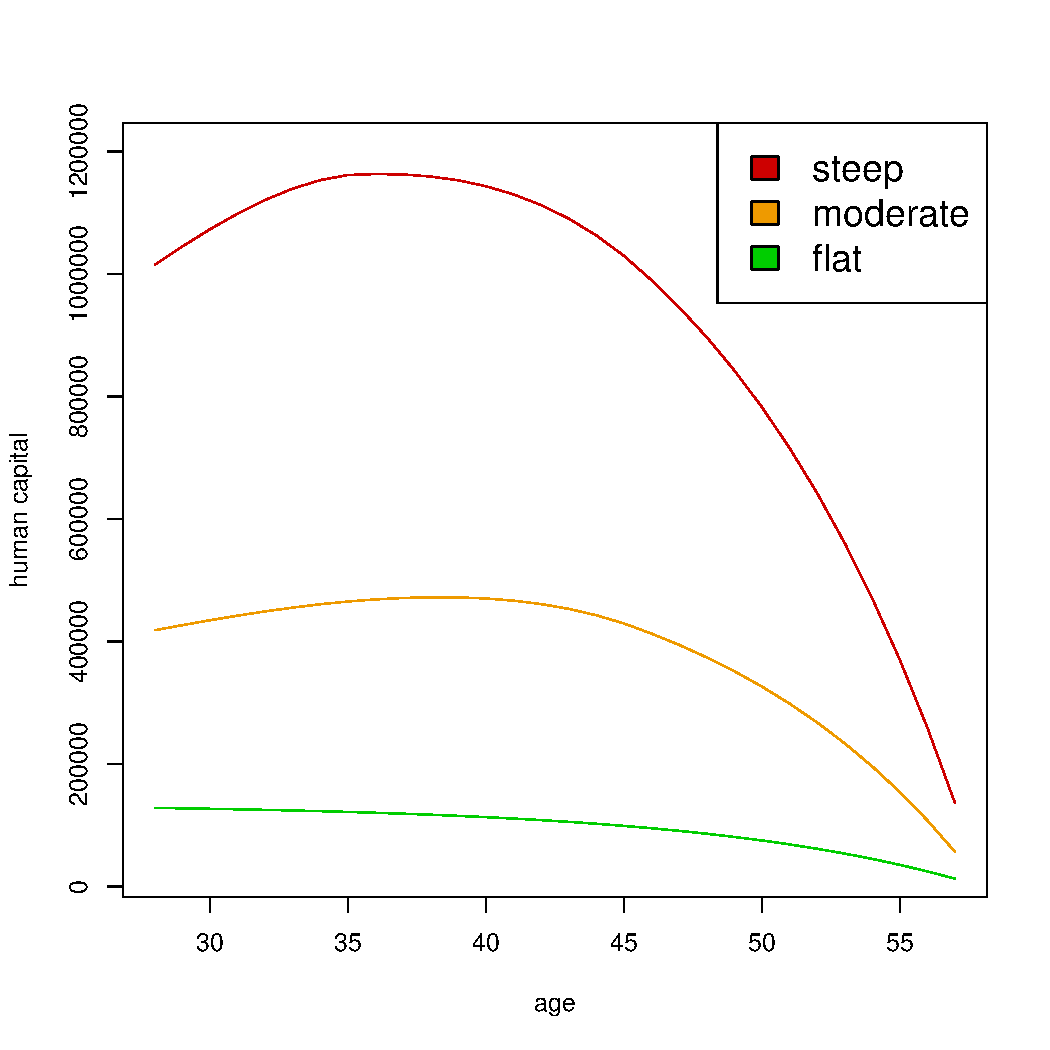
\includegraphics[scale=0.5]{figs/humancapital.pdf}
    \caption{Caption should be below the figure and not capitalized.}
\end{figure}


\begin{table}
	\centering
	\caption{Table Captions Should be Capitalized and Above Table}
	\begin{tabular}[H]{lc}
		\hline
		Fund name&Fund size\\
		\hline
		Anadolu Hayat Emeklilik&8.7 bln\\
		Garanti Emeklilik ve Hayat&7.4 bln\\
		AvivaSA Emeklilik ve Hayat&9.1 bln\\
		Allianz Yasam ve Emeklilik&6.8 bln\\
		Vakif Emeklili&3.5 bln\\
		\hline
	\end{tabular}\\
	Source: Pension Monitoring Center (2016)
\end{table}
